
% Document class options:
% =======================
% blind: Anonymise all author, affiliation, correspondence %        and funding information.
%
% lineno: Adds line numbers.
%
% serif: Sets the body font to be serif. 
%
% twocolumn: Sets the body text in two-column layout. 
% 
% num-refs: Uses numerical citation and references style 
%           (Vancouver-authoryear).
%
% alpha-refs: Uses author-year citation and references style %             (rss).
%
% Using other bibliography styles:
% =======================
%
% To specify a different bibiography style %
% 1) Do not use either num-refs or alpha-refs in documentclass.
% 2) Load natbib package with the options set as needed.
% 3) Use the \bibliographystyle command to specify the style % 
% Included NJD styles are: 
%   WileyNJD-ACS %   WileyNJD-AMA %   WileyNJD-AMS %   WileyNJD-APA %   WileyNJD-Harvard %   WileyNJD-VANCOUVER %
% or you may upload an alternative .bst file 
% (if requested by the journal).
%
% Examples:
% =======================
%% Example: Using numerical, sort-by-authors citations.
\documentclass[serif, twocolumn, authordate, meta]{jote-article}

\addbibresource{kristel.bib}



%% Example: Using author-year citations and anonymising submission % \documentclass[blind,alpha-refs]{wiley-article}

%% Example: Using unsrtnat for numerical, in-sequence citations % \documentclass{wiley-article}
% \usepackage[numbers]{natbib}
% \bibliographystyle{unsrtnat}

%% Example: Using WileyNJD-AMA reference style and superscript %%          citations, two-column and serif fonts for AIChE % \documentclass[serif,twocolumn,lineno]{wiley-article}
% \usepackage[super]{natbib}
% \bibliographystyle{WileyNJD-AMA}
% \makeatletter % \renewcommand{\@biblabel}[1]{#1.}
% \makeatother 
% Add additional packages here if required \usepackage{siunitx}


\usepackage{float}
\usepackage{bookmark}
\usepackage{lipsum}



% Use upquote if available, for straight quotes in verbatim environments



% Correct order of tables after \paragraph or \subparagraph

\makeatletter
\patchcmd\longtable{\par}{\if@noskipsec\mbox{}\fi\par}{}{}
\makeatother
% Allow footnotes in longtable head/foot

% Update article type if known % Include section in journal if known, otherwise delete \papertype{?}

\title{Burst Beliefs – Methodological Problems in the Balloon Analogue Risk Task and Implications for Its Use}

\papertype{Meta-research}

% List abbreviations here, if any. Please note that it is preferred that abbreviations be defined at the first instance they appear in the text, rather than creating an abbreviations list.
%\abbrevs{ABC, a black cat; DEF, doesn't ever fret; GHI, goes home immediately.}

% Include full author names and degrees, when required by the journal.
% Use the \authfn to add symbols for additional footnotes and present addresses, if any. Usually start with 1 for notes about author contributions; then continuing with 2 etc if any author has a different present address.
\author[1]{Kristel De Groot}

%Please also enter the authors in the same order here, for metadata purposes. This is a workaround.

\authorone{Kristel De Groot}
%\authorfour{}
%\authorfive{}
\runningauthor{De Groot}
%\contrib[\authfn{1}]{Equally contributing authors.}

% Include full affiliation details for all authors
\affil[1]{Erasmus University Rotterdam Institute for Behaviour and Biology (EURIBEB) |\newline Institute of Psychology, Erasmus School of Social and Behavioural Sciences |\newline Department of Applied Economics, Erasmus School of Economics;\newline Erasmus University Rotterdam, the Netherlands}

%\affil[2]{Department, Institution, City, State or Province, Postal Code, Country}

\corraddress{Kristel De Groot, Department of Psychology, Education \& Child Studies/ Research Methods and Techniques, Erasmus University, Rotterdam, the Netherlands}
\corremail{\href{mailto:k.degroot@ese.eur.nl}{k.degroot@ese.eur.nl}}

\funding{
    \begin{wrapfigure}[3]{l}{0.01\marginparwidth}
         \vskip-14pt
         
\includegraphics[height=3.7em]{media/NWO-logo huisstijlsite.png}
    \end{wrapfigure}    
    The author is supported by the Research Talent programme with project number $406.17.505$, which is financed by the Dutch Research Council (NWO).
     
    }

\acknowledgments{The author would like to acknowledge Jan van Ours, Marco Lauriola, and Sander Wieman for their constructive feedback on previous versions of this manuscript, and for sharing their views on the strengths and weaknesses of the BART. The author also expresses gratitude to Sander Wieman for his thorough language-editing and for proofreading the final manuscript.}

%\presentadd[\authfn{2}]{Department, Institution, City, State or Province, Postal Code, Country}

\paperdoi{10.36850/mr1}

% Include the name of the author that should appear in the running header \runningauthor{de Groot}

\jname{Journal of Trial and Error}
\jyear{2020}
\jvolume{1}
\jissue{1}
\jwebsite{https://www.jtrialerror.com}
\paperreceived{8 June 2020}
%\paperrevised{May 18th 2020}
\paperaccepted{31 August 2020}
\paperpublished{8 October 2020}
%Enter the date of publication in YYYY-MM-DD format (for CrossMark)
\paperpublisheddate{2020-11-23}
\jpages{43-51}
\jlogo{media/jote_logo_full}

\pubpub{https://archive.jtrialerror.com/pub/alcoholcues}
%\companionurl{}
%\companiontitle{}
%\companionabstract{}

%\keywords{alcohol, automatic cognition, gender stereotypes, lexical decision task, sexual aggression}

%\abstracttext{Alcohol and its effects on aggression have been the subject of many discussions and research papers. Despite this fact, there is still a debate surrounding what it is exactly about alcohol that causes aggression. The current study sought to replicate the past finding by Bartholow \& \textcite{Heinz2006}, that alcohol cues without consumption increase the accessibility of aggressive thoughts, which can then influence aggressive behaviors. In the present study, participants had to complete a lexical decision task that was set up to assess whether aggressive words were detected faster in the presence of alcohol-related pictures compared to neutral pictures. The results of this study did not replicate the expected finding as only a main effect of word type was found in which participants detected neutral words faster than aggressive words. Furthermore, the study aimed to assess the role of gender stereotype acceptance levels in this association, but due to faulty design considerations, such analyses were not possible. The results are discussed in terms of the limitations of the study, and propositions for future directions are addressed.}

%\rolling{YES}

%Controls the width and height of the abstract. Keep difference between these 5 for nice looking things.
\heightabstract{50mm}
\widthaffil{45mm}

\setlength{\parskip}{0pt}

%\contributions{\lipsum[1]}

\keywordsabstract{Balloon Analogue Risk Task, risk-taking, uncertainty, expected value, confounding, censoring.}


\begin{document}
\setcounter{page}{43}
\pdfbookmark[0]{De Groot, K. - Burst Beliefs – Methodological Problems in the Balloon Analogue Risk Task and Implications for Its Use}{Burst Beliefs – Methodological Problems in the Balloon Analogue Risk Task and Implications for Its Use}
\begin{frontmatter}
\maketitle 
\begin{abstract}
%\phantomsection %\addcontentsline{toc}{section}{Abstract}

\noindent Studies in the field of psychology often employ (computerized) behavioral tasks, aimed at mimicking real-world situations that elicit certain actions in participants. Such tasks are for example used to study risk propensity, a trait-like tendency towards taking or avoiding risk. One of the most popular tasks for gauging risk propensity is the Balloon Analogue Risk Task \parencite[BART;][]{Lejuez2002}, which has been shown to relate well to self-reported risk-taking and to real-world risk behaviors. However, despite its popularity and qualities, the BART has several methodological shortcomings, most of which have been reported before, but none of which are widely known. In the present paper, four such problems are explained and elaborated on: a lack of clarity as to whether decisions are characterized by uncertainty or risk; censoring of observations; confounding of risk and expected value; and poor decomposability into adaptive and maladaptive risk behavior.

Furthermore, for every problem, a range of possible solutions is discussed, which overall can be divided into three categories: using a different, more informative outcome index than the standard average pump score; modifying one or more task elements; or using a different task, either an alternative risk-taking task (sequential or otherwise), or a custom-made instrument. It is important to make use of these solutions, as applying the BART without accounting for its shortcomings may lead to interpretational problems, including false-positive and false-negative results. Depending on the research aims of a given study, certain shortcomings are more pressing than others, indicating the (type of) solutions most needed. By combining solutions and openly discussing shortcomings, researchers may be able to modify the BART in such a way that it can operationalize risk propensity without substantial methodological problems.
\end{abstract}
\end{frontmatter}


\phantomsection
\addcontentsline{toc}{section}{Purpose}
\section*{Purpose}
The Balloon Analogue Risk Task (BART) is one of the most widely used behavioral tasks in psychology and has an especially strong presence in the fields of decision research, addiction research, and neuropsychology. But despite its popularity, researchers using the BART seem largely unaware of the task's methodological shortcomings, which sometimes leads to conclusions that are not supported by the data. This is likely a result of these shortcomings not being widely reported, as "failure" is not considered a popular publishing theme. Therefore, the present paper aims to gather and review these shortcomings, as well as potential solutions.

\phantomsection
\addcontentsline{toc}{section}{Take-home Message}
\section*{Take-home Message}
The Balloon Analogue Risk Task (BART) suffers from various methodological shortcomings. The present paper analyses these shortcomings and offers suggestions to mitigate their effects. Finally, it calls upon researchers to critically evaluate how these shortcomings impact their studies before deciding whether and how to use BART.

\phantomsection
\addcontentsline{toc}{section}{Introduction}
\section*{Introduction}

To a large extent, psychological science rests on the promises of operationalization: defining fuzzy concepts as measurable variables, or in other words, changing conceptual variables into operational ones \parencite{Shuttleworth2008}. This process is imperative because most concepts researchers hypothesize about are not straightforwardly quantifiable. By defining how a concept is measured, operationalization allows hypotheses to take a falsifiable format and enables us to replicate findings. In a way, operationalizations are arbitrary, as concepts can be defined and thus measured in numerous ways -- none of which are surely "right".
Nonetheless, some measures may be more suitable than others.

A notable example of a concept that can be operationalized in various ways is risk-taking \parencite{Lauriola2018}, which has an important place in clinical, cognitive, and developmental psychology, as well as in the fields of criminology, economics, and management. One way risk-taking is operationalized in these fields is through self-report measures, such as the Domain-Specific Risk-Taking (DOSPERT) scale \parencite{Blais2006} and the Financial Risk Tolerance assessment \parencite{Grable1999}. Another way is through computerized behavioral tasks, like the Iowa Gambling Task \parencite{Bechara1994}, the Cambridge Gambling Task \parencite{Rogers1999}, the Game of Dice Task \parencite{Brand2005}, the Balloon Analogue Risk Task \parencite{Lejuez2002}, and the more recent but already widely used Columbia Card Task \parencite{Figner2009}. Importantly, the quality of a study largely depends on the degree to which its operational measures reflect the underlying concept; in this case, one's disposition towards risk-taking. If a task is a poor proxy for a concept or is subject to methodological or interpretational problems, any data resulting from it are of limited value to our understanding of the concept. In this regard, several studies have challenged the operationalization ability of the most-cited risk task, the Iowa Gambling Task \parencite[see e.g.,][]{Brand2006, Buelow2009, Figner2009, Maia2004}. The Balloon Analogue Risk Task, which is the second-most cited, may yet suffer from even more severe issues, hindering its ability to operationalize risk-taking. While some individual issues have been reported in previous publications, no literature so far has discussed these collectively. The present commentary aspires to fill this gap.

\phantomsection
\addcontentsline{toc}{section}{The Balloon Analogue Risk Task}
\section*{The Balloon Analogue Risk Task}

In the Balloon Analogue Risk Task, or BART for short, participants are presented with a computer screen showing a small balloon and a pump. They are told that every time they click the pump, the balloon expands, and a fixed amount of money (5 cents) is added to a temporary bank. Every pump also increases the chance of the balloon exploding (marked by a "pop" sound from the computer), resulting in losing all money in the temporary bank for that particular balloon (trial). The point at which a balloon explodes varies across trials, ranging from the first pump to the point where the balloon fills the entire screen. Participants can decide to stop pumping the balloon at any point during a trial by clicking the "collect" button (left in Figure \ref{fig:figure1}), which transfers the money accumulated in their temporary bank to their permanent one, while a slot machine sound is played. Once a balloon explodes or once participants cash a balloon's proceeds, the trial ends, and a new, uninflated, balloon appears.

In the original study by \textcite{Lejuez2002}, participants were informed that they would complete 90 balloons: 30 orange, 30 yellow, and 30 blue ones. Unbeknownst to participants, differently colored balloons had a different chance of exploding. The probability distribution governing their explosion points consisted of an array of \(n\) numbers from which on every pump a random number was drawn without replacement. If a 1 was drawn, the balloon exploded.

\noindent\begin{minipage}{.48\textwidth}
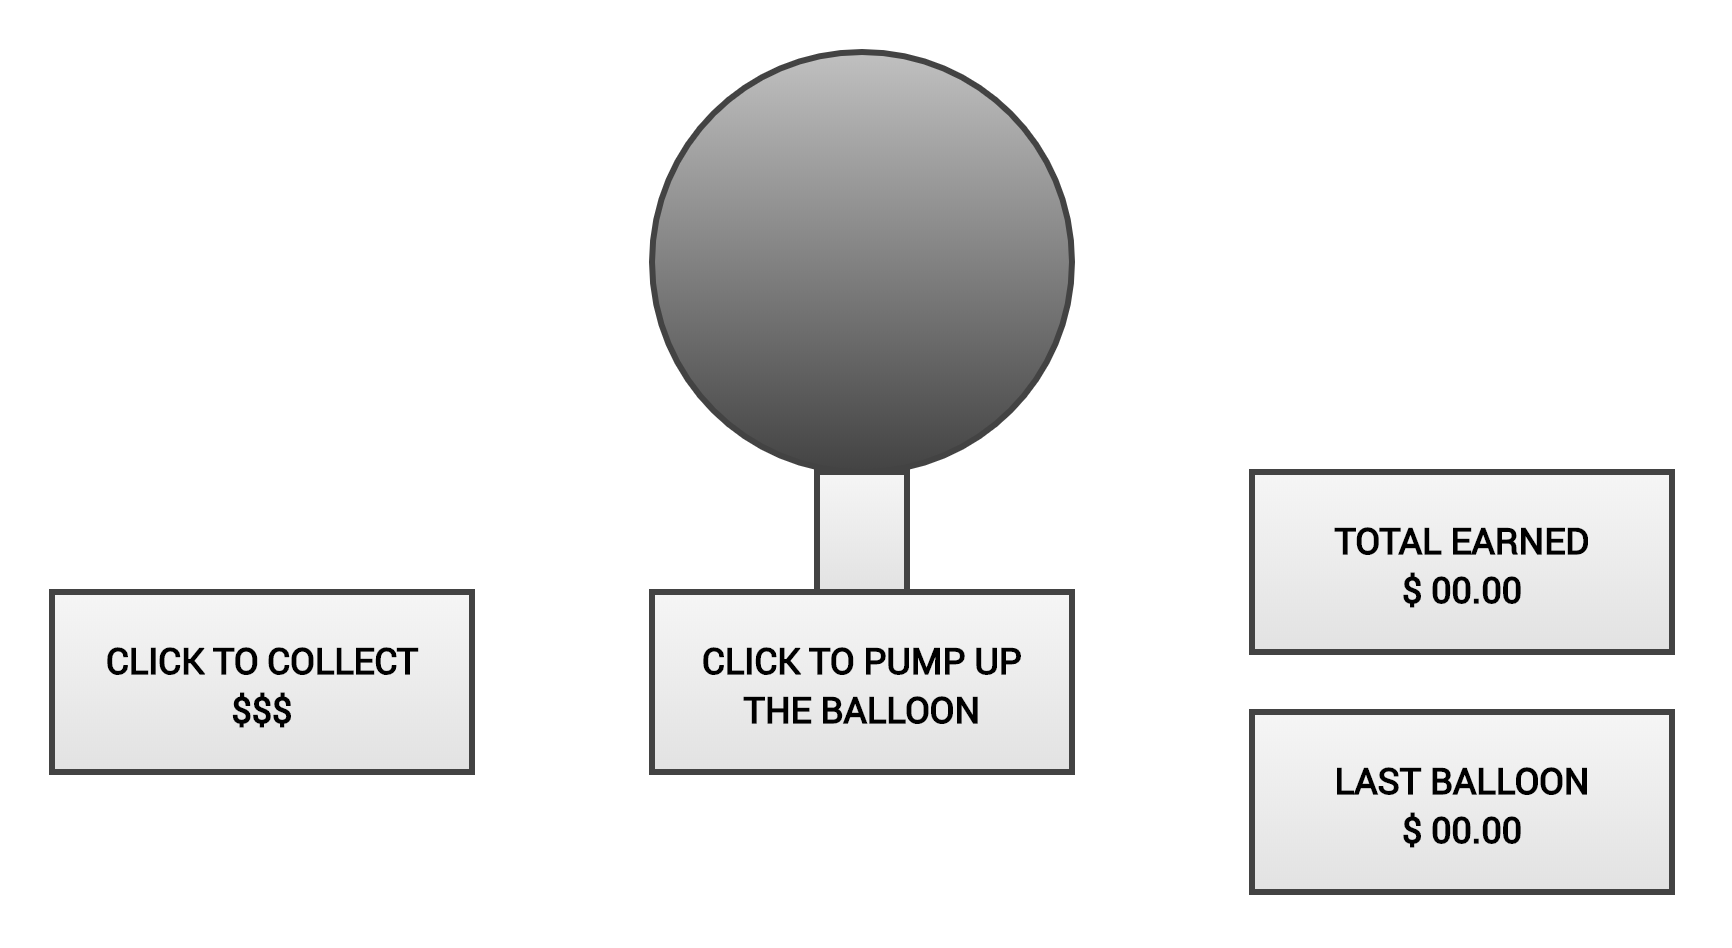
\includegraphics[width=\textwidth]{media/Anonymised Figure_1 - BART Problems (1).png}
\captionof{figure}{Set-up of the original Balloon Analogue Risk Task as described by \textcite{Lejuez2002}. An interactive illustration of the task is provided with \href{https://archive.jtrialerror.com/pub/burstbeliefs/\#the-balloon-analogue-risk-task}{the HTML version of this article.}}
\label{fig:figure1}
\end{minipage}

\vspace*{1\baselineskip}

Thus, the probability \(p\) of the balloon exploding on the first pump was \(1/n\), and the probability of it exploding on pump \(i\) (given no prior explosion) was \(p_{i} = \ \frac{1}{n\  - \ i\  + \ 1}\). For orange balloons, the array ranged from 1 to 8 (hence \(p_{1} = \frac{1}{8 - 1 + 1} = 1/8\)), for yellow balloons from 1 to 32 (\(p_{1} = \frac{1}{32 - 1 + 1} = 1/32\)), and for blue ones from 1 to 128 (\(p_{1} = \frac{1}{128 - 1 + 1} = 1/128\)). Their average explosion points were respectively 4, 16, and 64, with the same (randomly generated) sets of explosion points being used across all participants to limit extraneous variability. Neither the ranges nor the average explosion points were communicated to participants.

The BART's design is intended to reflect naturalistic decision-making, in which taking more risk generally increases the odds of encountering a loss. This sort of decision-making tends to be emotionally engaging, instigating a sense of increasing tension as the balloon increases in size \parencite{Schonberg2011}. In support of the BART's validity, \textcite{Lejuez2002} showed that the average number of times participants pumped the blue balloon significantly correlated with scores on risk-related constructs (sensation seeking, impulsivity) and with real-world risk behaviors, such as polydrug use, gambling, unsafe sex, and stealing. The orange and yellow pumps were originally not examined with respect to risk-related constructs, as their narrow ranges of outcome values (1-8 and 1-32) are less suited for capturing individual differences. Instead, their average pump numbers were analyzed together with those of the blue balloons to show that the number of times participants choose to pump is sensitive to the probability of exploding. Overall, the data showed the BART to have ``particular promise as a behavioral index of risk-taking'' \parencite[p. 82]{Lejuez2002}. As would be expected based on this conclusion, the BART (particularly its blue balloon) became a popular instrument for gauging individuals' propensity for risk-taking, with inconsistent findings being attributed to factors like sampling variability and inadequate statistical power \parencite{Lauriola2014}, rather than problems inherent to the BART. However, several authors have argued that such problems exist \parencite{deGroot2018, Gu2018, Schmidt2019, Schonberg2011}, and that they limit the BART's ability to measure one's propensity for taking risk. The key problems that characterize the BART are 1) a lack of clarity as to whether decisions are characterized by uncertainty or risk, 2) censoring of observations, 3) confounding of risk and expected value, and 4) poor decomposability into adaptive and maladaptive risk behavior.

\phantomsection
\addcontentsline{toc}{subsection}{Risk or Uncertainty?}
\subsection*{Risk or uncertainty?}
\label{sec:risk}

In economic theories of decision-making, a key distinction is that between uncertainty and risk, which is often accredited to \textcite{Knight1921}, and was introduced to psychological thinking in a seminal paper by \textcite{Edwards1954} that lies at the origin of behavioral decision theory. When deciding under the condition of risk, the probabilities associated with the possible outcomes are \emph{known}. When deciding under uncertainty (which some authors call ambiguity), this probability distribution is \emph{unknown}.

For \textcite{Knight1921}, this distinction was not only of theoretical but of practical importance as well. According to him, uncertainty -- not risk -- was the main driver of entrepreneurial success, as only people who recognize hidden opportunities can seize them and profit from them. Since then, the empirical relevance of the uncertainty-risk distinction has been confirmed in various fields of research. In economics, \textcite{Ellsberg1961} showed that individuals prefer risk over uncertainty, even if the known probabilities are unfavorable and the uncertain option could be a guaranteed win. In psychology, studies showed that uncertain and risky decisions involve different mental processes, as risk allows for statistical thinking (to optimize) but uncertainty involves heuristics (to satisfice) \parencite{Volz2012}. In line with this, decision-making under risk is thought to depend more on executive function (such as categorization and cognitive flexibility) for which the dorsolateral prefrontal cortex is important, whereas decision-making under uncertainty hinges on emotional processes (such as somatic feedback), which are more associated with the ventromedial prefrontal cortex and the amygdala \parencite{Brand2006}. This may explain why patients with executive deficits, such as those with Parkinson's disease, have difficulty deciding under risk but have no trouble deciding under uncertainty \parencite{Euteneuer2009}, whereas persons with obsessive-compulsive disorder, for example, show the opposite pattern \parencite{Starcke2009, Starcke2010}.

Given that uncertainty and risk differ both theoretically and empirically, it is imperative for researchers to know the conditions under which participants decide. Unfortunately, despite the word "risk" in its name, these conditions are not straightforward in the BART. Since participants are never given "detailed information about the probability of an explosion'' \parencite[p. 77]{Lejuez2002}, we can assume that at least during early trials, they decide under uncertainty \parencite{Bishara2009, deGroot2018, Schonberg2011}. As they move further along in the task and "sample the distribution" by pumping balloons and observing their outcomes, they get a better sense of the probabilities, which gradually moves their decisions in the direction of risk. Although not studied in the BART itself, such a shift has been shown for the Iowa Gambling Task, where performance in early trials does not correlate with that in later trials nor with executive function, indicating that people first decide under uncertainty and later under risk \parencite{Brand2006,Brand2007}. While this effect may not be as strong in the BART, studies do show better performance in later compared to early trials, suggesting that participants indeed get a better grasp of the probability distribution over time \parencite{Lejuez2002,deGroot2019}.\footnote{The relevant data collected by \cite{deGroot2019} on per-block averages is not reported in the published report but will be shared upon request.}

The BART's transition from uncertainty towards risk is problematic for several reasons. First, it is unclear \emph{when} exactly this shift transpires, making it difficult to determine whether a decision in a given trial is made under uncertainty, risk, or something in between. Second, the point where decisions shift from uncertainty to risk is likely to differ between individuals, and is dependent on task characteristics \parencite{Brand2006,Brand2007}. Third, the shift implies that the BART imposes learning demands, which could inadvertently impact participants' outcomes on the task, with those capable of updating their knowledge of the probabilities performing better than those who have difficulty doing so. Fourth, once participants manage to derive the task's probabilities, subsequent decisions are not characterized by what is usually considered risk. Contrary to decisions in which probabilities are explicitly described ("a priori" probabilities), probabilities in the BART are derived from experience. Since such probabilities depend on factors like sampling variability and one's memory of previous events, decision-makers treat experience-based probability differently, which is called the description-experience gap \parencite{Hau2008,Rakow2010}. Most notably, when deciding based on experience, people do not act in accordance with prospect theory, but instead, underweight rare events and overweight common encounters. As people have more and more encounters (e.g., trials), their experiences will approach the precision of a priori probabilities, though in practice this is difficult to attain \parencite{Knight1921}.

\label{sec:riskp5}
To address the inability of the BART to differentiate between complete uncertainty, experience-based risk, and description-based risk, several approaches may be used. One option is to apply a model to the BART's data that allows for participants learning through experience. An early example is a model by \textcite{Wallsten2005} in which decision-makers update their probabilities from trial to trial, and continually re-evaluate their options. Alternatively, one could use a different task, in which decisions are either all characterized by uncertainty or risk, or which includes a well-understood shift between the two. Tasks that involve only uncertain decision-making are rather difficult to design, as they require participants to be ignorant of probability-related information and \emph{remain} ignorant of that as well -- automatically disqualifying tasks that have a learning curve. Tasks involving only decisions made under (a priori) risk are much more common and include the Cambridge Gambling Task, the Game of Dice Task, and the Columbia Card Task, the latter of which resembles the BART's dynamic, affective nature \parencite{Schonberg2011}. Finally, a known shift from uncertainty to (experience-based) risk can be found in the Iowa Gambling Task. This task's shift, while not \emph{fully} understood, has been studied more thoroughly than that in the BART.

\phantomsection
\addcontentsline{toc}{subsection}{Censored Observations}\subsection*{Censored observations}

Statistical censoring refers to a condition in which the value of an observation is unknown because it is beyond a certain limit. This limit can exist by design, which is common in survival analysis. If a study on a surgical intervention follows patients for up to 10 years, the longevity scores of those who live past this term are censored, as their longevity is \emph{at least} 10 \parencite{Young2019}. Censoring can also result from limits on what an instrument can reliably measure. For example, the full IQ score of the Wechsler Adult Intelligence Scale ranges from 40 to 160 \parencite{Sattler2009}, meaning that IQ scores of people performing either extremely poorly or extremely well are cut off at these boundaries and are thus censored.

In the BART, censoring (by design) occurs if a participant is stopped from taking more risk in a given trial, because the balloon they are pumping explodes, forcing the trial to end. Since such a trial ends prematurely, the number of times the participant pumped the balloon does not necessarily reflect the risk they were willing to take, meaning their risk propensity is censored. This is problematic for various reasons. First, including these censored trials biases the average number of pumps downwards (especially for high-risk takers), underestimating participants' willingness to take risks \parencite{Dijkstra2020,Pleskac2008}. Likewise, the between-subjects variability across these averages is reduced \parencite{Lejuez2002}. Overall, the (unadjusted) average number of pumps is an ill-suited operationalization of risk propensity.

As censoring affects all sequential risk-taking tasks like the BART (involving multiple decisions per trial) and various other research paradigms, like survival analysis, several solutions have been proposed. In the paper introducing the BART, \textcite{Lejuez2002} suggest computing an adjusted pump average using only trials in which participants stopped voluntarily, that is, in which the balloon did not burst. However, by omitting explosion trials, censored observations are essentially treated as randomly missing, which is inaccurate \parencite{Pleskac2008}. The more risk someone takes, the more likely it is that the balloon bursts, and that the trial forcibly ends. The termination of trials is therefore not independent from participants' behavior. As a result, Lejuez et al.'s adjusted score tends to discard trials in which participants take a lot of risk. This causes the average number of pumps to be biased downwards, similar to the unadjusted score, but to a lesser extent.


\renewcommand{\thefootnote}{\fnsymbol{footnote}}
To circumvent the problem of censoring, \textcite{Pleskac2008} developed an automatic response version of the BART.\footnote{An interactive illustration of this task is provided with  \href{https://archive.jtrialerror.com/pub/burstbeliefs/\#censored-observations}{the HTML version of this article.}} Contrary to the standard BART, in which participants inflate a balloon one pump at a time, the automatic BART lets them indicate their intended number of pumps beforehand. The balloon then inflates to the corresponding size, or until it bursts. This procedure allows for an unbiased statistic of risk propensity, as the intended number of pumps is now observable in all trials \parencite{Pleskac2008}. However, it increases the time between decision and outcome, which may make decisions less emotional (impulsive) and more cognitive (planned) \parencite{Pleskac2008}, and may reduce the salience of the outcomes. These effects, in turn, can affect participants' risk-taking \parencite{Young2019}. In contrast, however, a study using the Bomb Risk Elicitation Task \parencite[BRET; ][]{Crosetto2013}, another risk task that uses delayed explosions to circumvent censoring, found that introducing such delays did not impact risk-taking.


\renewcommand{\thefootnote}{\arabic{footnote}}
Another solution to censoring is using a rigged task \parencite{Slovic1966}. Participants are then told that failure can occur at any moment (in the BART, at any pump), but actually, it is set to occur at the last possible choice. Hence, participants can always stop voluntarily, and no scores are censored. To uphold credibility, "mock" trials are added, in which failure is set to occur early on. Deciding on the number and timing of mock trials, however, is a challenge. Since behavior in a trial is affected by previous outcomes, experiencing (too) few failures could increase risk-taking \parencite{deGroot2019,Dijkstra2020}. Therefore, rigged tasks should be designed such that they produce failure rates similar to non-rigged tasks and should take into account that failure rates differ between participants too. However, research on the Columbia Card Task, another sequential risk-taking task, shows that this is often not the case \parencite{deGroot2019}.

A final remedy, which addresses the bias but leaves the BART unchanged, is to apply a statistical model to the resulting data that explicitly incorporates censored behavior. Such models consider \emph{all} observed data, using the censored trials as lower bounds in determining a participant's actual risk propensity. Some of them employ Bayesian (generalized) linear mixed-effects regression \parencite{Weller2019, Young2019}; others use maximum likelihood estimation, adding a cumulative distribution function to the likelihood function to account for censoring \parencite{Dijkstra2020,Tobin1958}. Such models perform significantly better (i.e., have less biased predictions) than those that do not account for censoring. However, as is the case for all statistical models, their soundness hinges on the validity of their underlying assumptions \parencite{Schafer2002}, such as that of normality, whose violation not all models are robust against \parencite{Powell1984}.

\phantomsection
\addcontentsline{toc}{subsection}{Confounding and Decomposability}
\subsection*{Confounding and decomposability}
\label{sec:confounding}

The BART was designed to resemble real-world risk situations, where taking modest risk is generally advantageous, but taking excessive risk is increasingly unfavorable \parencite{Lejuez2002,Wallsten2005}. Within a trial, every successful pump earns participants 5 cents, which are added to their temporary bank. As the amount accumulated in the bank grows, the relative gain of taking additional risk decreases, while the potential loss in case of an explosion increases. Additionally, the probability of the balloon exploding increases with every pump: from 1/128 on the first to 1/127 on the second, and so on.
\label{sec:confoundingp2}
This combination of characteristics makes that the task's structure entails a serious problem. Since both the balloon value (the amount collected in the temporary bank) and the explosion probability increase with every pump, the expected value of inflating the balloon -- the product of the success chance and the reward, minus the product of the explosion chance and the balloon value -- changes across a trial \parencite{Schmidt2019}. This change is illustrated in Table \ref{tab:table1}. Early in a trial, the expected value of the pump is positive, so taking additional risk is advantageous. This prospect changes halfway when the expected value turns negative, making additional pumps unfavorable \parencite{Lejuez2002}. Due to the expected value changing with each decision, it is \emph{confounded} with risk (defined as the variability of the possible outcomes), which varies across decisions by design. Although such confounding can happen in real-life decision-making, it is not desirable in a controlled scientific environment: it makes it difficult to measure participants' risk propensity, as both risk and expected value may influence their decisions. The extent to which individuals are, for example, risk-seeking, can therefore not be determined, because this would require showing a preference for higher variance payoffs, holding expected value constant \parencite{Schonberg2011}.

This confounding demonstrates that the BART's main observable outcome -- the number of pumps participants press -- cannot be interpreted as a straightforward indicator of risk propensity. Like many behavioral tasks, the BART supposedly gauges a single cognitive construct, but it manipulates various other, potentially confounding constructs as well \parencite{Schonberg2011}. Expected value is an example of such a construct. As a result, the single score provided by the BART cannot easily be decomposed to identify the cognitive or neural mechanisms involved in the pump decisions. Studying the risk-taking process in isolation using the BART is therefore not possible.

One approach for resolving the confounding and decomposability issues in the BART is to apply a computational model to its data that quantifies the cognitive mechanisms underlying the observed behavior \parencite{Bishara2009}. Such models were first proposed by \textcite{Wallsten2005}, inspired by an expectancy-valence model for decomposing behavior in the Iowa Gambling Task \parencite{Busemeyer2002}.  \textcite{Wallsten2005} explain decision variability using one parameter for risk-taking, one for response consistency, and two for learning. By applying these models, we can study risk-taking -- and other aspects that determine BART behavior -- in isolation, by translating "what is observed but relatively uninformative to what is unobserved and relatively informative" \parencite[p. 95]{vanRavenzwaaij2011}. However, data from the BART may not be rich enough to warrant the use of complicated decomposition models. For instance, a study on Wallsten et al.'s best performing model demonstrated that its learning parameters could not reliably be recovered \parencite{vanRavenzwaaij2011}. To allow for more extensive decomposition, one may need to resort to a different task, like the Iowa Gambling Task. Alternatively, one could use a task that by design avoids confounding, such as the Columbia Card Task. Although dynamic and affective like the BART, this task orthogonally varies risk-related constructs, so that they can be decomposed into their underlying mechanisms -- like sensitivity to gains, losses, and probabilities -- without the use of a computational model \parencite{Dijkstra2020, Figner2009, Schonberg2011}. Finally, researchers can choose to design a custom task to ensure that the constructs relevant to their hypotheses are not confounded. For example, a risk task presented in \textcite{Schmidt2013} varies the level of risk but holds expected value constant. Solutions such as these should be considered carefully so that constructs crucial to a study's hypotheses can be isolated effectively.

\phantomsection
\addcontentsline{toc}{subsection}{The Normative Solution}
\subsection*{The normative solution}
\label{sec:normative}

The BART is designed in such a way that the balloons' average explosion point lies at 64, halfway the maximum number of pumps. This is achieved by randomly generating collections of explosion points until one produces an average of 64 over all trials, as well as within each set of 10 trials \parencite{Lejuez2002}. Participants can then maximize their earnings by attempting to pump every balloon 64 times, which results in an explosion in about half of the trials, and an optimal overall expected value. Going back to \hyperlink{Table 1}{Table 1}, we can see exactly why this is the optimal, or \emph{normative}, solution in the BART. Up to and including the 64\textsuperscript{th} pump, the expected value of pumping the balloon is positive; after $64$, the expected value is (increasingly) negative. It is, therefore, optimal to aim for 64 pumps on every balloon, and then stop. Choosing to pump more \emph{or} fewer than 64 times will decrease expected earnings; and the farther one deviates from the optimum, the lower the expected earnings become \parencite{Lejuez2002, Pleskac2008, Wallsten2005}. Remarkably, in most trials, participants stop pumping the balloon far before the optimal stopping point \parencite{Lejuez2002}. In fact, the average adjusted pump score is typically between 26 and 35 \parencite{Pleskac2008}. Real-world risk-avoiders and risk-takers alike rarely pump the balloon enough times to maximize their expected earnings. This is less of a problem in the automatic BART, although participants there still pump fewer than 64 times on average. For example, two recent studies reported averages of 61.9 \parencite{Bernoster2019} and 58.5 pumps \parencite{deGroot2019}.


\begin{table*}[ht]\sffamily
\begin{tabular}{@{}lllllll@{}}
\hline \noalign{\vskip 2mm}      
\begin{minipage}[b]{0.12\linewidth}\raggedright \textbf{Pump Number}

\textbf{(A)}\strut \end{minipage} & \begin{minipage}[b]{0.12\linewidth}\raggedright \textbf{Balloon Value Before Pump}

\textbf{(B)}\strut \end{minipage} & \begin{minipage}[b]{0.12\linewidth}\raggedright \textbf{Balloon Value After Pump}

\textbf{(C)}\strut \end{minipage} & \begin{minipage}[b]{0.12\linewidth}\raggedright \textbf{Chance of Explosion}

\textbf{(D)}\strut \end{minipage} & \begin{minipage}[b]{0.12\linewidth}\raggedright \textbf{Chance of Success}

\textbf{(E)}\strut \end{minipage} & \begin{minipage}[b]{0.12\linewidth}\raggedright \textbf{Expected Value of Current Pump}

\textbf{(F)}\strut \end{minipage} & \begin{minipage}[b]{0.12\linewidth}\raggedright \textbf{Expected Value of All Remaining Pumps (G)}\strut \end{minipage}\tabularnewline \hline \begin{minipage}[t]{0.12\linewidth}\raggedright 1\strut \end{minipage} & \begin{minipage}[t]{0.12\linewidth}\raggedright € -\strut \end{minipage} & \begin{minipage}[t]{0.12\linewidth}\raggedright € 0.05\strut \end{minipage} & \begin{minipage}[t]{0.12\linewidth}\raggedright 0.00781\strut \end{minipage} & \begin{minipage}[t]{0.12\linewidth}\raggedright 0.99219\strut \end{minipage} & \begin{minipage}[t]{0.12\linewidth}\raggedright € 0.04961\strut \end{minipage} & \begin{minipage}[t]{0.12\linewidth}\raggedright € 1.60000\strut \end{minipage}\tabularnewline \begin{minipage}[t]{0.12\linewidth}\raggedright 2\strut \end{minipage} & \begin{minipage}[t]{0.12\linewidth}\raggedright € 0.05\strut \end{minipage} & \begin{minipage}[t]{0.12\linewidth}\raggedright € 0.10\strut \end{minipage} & \begin{minipage}[t]{0.12\linewidth}\raggedright 0.00787\strut \end{minipage} & \begin{minipage}[t]{0.12\linewidth}\raggedright 0.99213\strut \end{minipage} & \begin{minipage}[t]{0.12\linewidth}\raggedright € 0.04921\strut \end{minipage} & \begin{minipage}[t]{0.12\linewidth}\raggedright € 1.56260\strut \end{minipage}\tabularnewline \begin{minipage}[t]{0.12\linewidth}\raggedright 3\strut \end{minipage} & \begin{minipage}[t]{0.12\linewidth}\raggedright € 0.10\strut \end{minipage} & \begin{minipage}[t]{0.12\linewidth}\raggedright € 0.15\strut \end{minipage} & \begin{minipage}[t]{0.12\linewidth}\raggedright 0.00794\strut \end{minipage} & \begin{minipage}[t]{0.12\linewidth}\raggedright 0.99206\strut \end{minipage} & \begin{minipage}[t]{0.12\linewidth}\raggedright € 0.04840\strut \end{minipage} & \begin{minipage}[t]{0.12\linewidth}\raggedright € 1.52540\strut \end{minipage}\tabularnewline \begin{minipage}[t]{0.12\linewidth}\raggedright 4\strut \end{minipage} & \begin{minipage}[t]{0.12\linewidth}\raggedright € 0.15\strut \end{minipage} & \begin{minipage}[t]{0.12\linewidth}\raggedright € 0.20\strut \end{minipage} & \begin{minipage}[t]{0.12\linewidth}\raggedright 0.00800\strut \end{minipage} & \begin{minipage}[t]{0.12\linewidth}\raggedright 0.99200\strut \end{minipage} & \begin{minipage}[t]{0.12\linewidth}\raggedright € 0.04840\strut \end{minipage} & \begin{minipage}[t]{0.12\linewidth}\raggedright € 1.48840\strut \end{minipage}\tabularnewline \begin{minipage}[t]{0.12\linewidth}\raggedright 5\strut \end{minipage} & \begin{minipage}[t]{0.12\linewidth}\raggedright € 0.20\strut \end{minipage} & \begin{minipage}[t]{0.12\linewidth}\raggedright € 0.25\strut \end{minipage} & \begin{minipage}[t]{0.12\linewidth}\raggedright 0.00806\strut \end{minipage} & \begin{minipage}[t]{0.12\linewidth}\raggedright 0.99194\strut \end{minipage} & \begin{minipage}[t]{0.12\linewidth}\raggedright € 0.04798\strut \end{minipage} & \begin{minipage}[t]{0.12\linewidth}\raggedright € 1.45161\strut \end{minipage}\tabularnewline \begin{minipage}[t]{0.12\linewidth}\raggedright (\ldots)\strut \end{minipage} & \begin{minipage}[t]{0.12\linewidth}\raggedright \strut \end{minipage} & \begin{minipage}[t]{0.12\linewidth}\raggedright \strut \end{minipage} & \begin{minipage}[t]{0.12\linewidth}\raggedright \strut \end{minipage} & \begin{minipage}[t]{0.12\linewidth}\raggedright \strut \end{minipage} & \begin{minipage}[t]{0.12\linewidth}\raggedright \strut \end{minipage} & \begin{minipage}[t]{0.12\linewidth}\raggedright \strut \end{minipage}\tabularnewline \begin{minipage}[t]{0.12\linewidth}\raggedright 62\strut \end{minipage} & \begin{minipage}[t]{0.12\linewidth}\raggedright € 3.05\strut \end{minipage} & \begin{minipage}[t]{0.12\linewidth}\raggedright € 3.10\strut \end{minipage} & \begin{minipage}[t]{0.12\linewidth}\raggedright 0.01493\strut \end{minipage} & \begin{minipage}[t]{0.12\linewidth}\raggedright 0.98507\strut \end{minipage} & \begin{minipage}[t]{0.12\linewidth}\raggedright € 0.00373\strut \end{minipage} & \begin{minipage}[t]{0.12\linewidth}\raggedright € 0.00672\strut \end{minipage}\tabularnewline \begin{minipage}[t]{0.12\linewidth}\raggedright 63\strut \end{minipage} & \begin{minipage}[t]{0.12\linewidth}\raggedright € 3.10\strut \end{minipage} & \begin{minipage}[t]{0.12\linewidth}\raggedright € 3.15\strut \end{minipage} & \begin{minipage}[t]{0.12\linewidth}\raggedright 0.01515\strut \end{minipage} & \begin{minipage}[t]{0.12\linewidth}\raggedright 0.98485\strut \end{minipage} & \begin{minipage}[t]{0.12\linewidth}\raggedright € 0.00227\strut \end{minipage} & \begin{minipage}[t]{0.12\linewidth}\raggedright € 0.00303\strut \end{minipage}\tabularnewline \begin{minipage}[t]{0.12\linewidth}\raggedright 64\strut \end{minipage} & \begin{minipage}[t]{0.12\linewidth}\raggedright € 3.15\strut \end{minipage} & \begin{minipage}[t]{0.12\linewidth}\raggedright € 3.20\strut \end{minipage} & \begin{minipage}[t]{0.12\linewidth}\raggedright 0.01538\strut \end{minipage} & \begin{minipage}[t]{0.12\linewidth}\raggedright 0.98462\strut \end{minipage} & \begin{minipage}[t]{0.12\linewidth}\raggedright € 0.00077\strut \end{minipage} & \begin{minipage}[t]{0.12\linewidth}\raggedright € 0.00077\strut \end{minipage}\tabularnewline \begin{minipage}[t]{0.12\linewidth}\raggedright 65\strut \end{minipage} & \begin{minipage}[t]{0.12\linewidth}\raggedright € 3.20\strut \end{minipage} & \begin{minipage}[t]{0.12\linewidth}\raggedright € 3.25\strut \end{minipage} & \begin{minipage}[t]{0.12\linewidth}\raggedright 0.01563\strut \end{minipage} & \begin{minipage}[t]{0.12\linewidth}\raggedright 0.98438\strut \end{minipage} & \begin{minipage}[t]{0.12\linewidth}\raggedright € -0.00078\strut \end{minipage} & \begin{minipage}[t]{0.12\linewidth}\raggedright € -0.00078\strut \end{minipage}\tabularnewline \begin{minipage}[t]{0.12\linewidth}\raggedright 66\strut \end{minipage} & \begin{minipage}[t]{0.12\linewidth}\raggedright € 3.25\strut \end{minipage} & \begin{minipage}[t]{0.12\linewidth}\raggedright € 3.30\strut \end{minipage} & \begin{minipage}[t]{0.12\linewidth}\raggedright 0.01587\strut \end{minipage} & \begin{minipage}[t]{0.12\linewidth}\raggedright 0.98413\strut \end{minipage} & \begin{minipage}[t]{0.12\linewidth}\raggedright € -0.00238\strut \end{minipage} & \begin{minipage}[t]{0.12\linewidth}\raggedright € -0.00238\strut \end{minipage}\tabularnewline \begin{minipage}[t]{0.12\linewidth}\raggedright (\ldots)\strut \end{minipage} & \begin{minipage}[t]{0.12\linewidth}\raggedright \strut \end{minipage} & \begin{minipage}[t]{0.12\linewidth}\raggedright \strut \end{minipage} & \begin{minipage}[t]{0.12\linewidth}\raggedright \strut \end{minipage} & \begin{minipage}[t]{0.12\linewidth}\raggedright \strut \end{minipage} & \begin{minipage}[t]{0.12\linewidth}\raggedright \strut \end{minipage} & \begin{minipage}[t]{0.12\linewidth}\raggedright \strut \end{minipage}\tabularnewline \begin{minipage}[t]{0.12\linewidth}\raggedright 124\strut \end{minipage} & \begin{minipage}[t]{0.12\linewidth}\raggedright € 6.15\strut \end{minipage} & \begin{minipage}[t]{0.12\linewidth}\raggedright € 6.20\strut \end{minipage} & \begin{minipage}[t]{0.12\linewidth}\raggedright 0.20000\strut \end{minipage} & \begin{minipage}[t]{0.12\linewidth}\raggedright 0.80000\strut \end{minipage} & \begin{minipage}[t]{0.12\linewidth}\raggedright € -1.19000\strut \end{minipage} & \begin{minipage}[t]{0.12\linewidth}\raggedright € -1.19000\strut \end{minipage}\tabularnewline \begin{minipage}[t]{0.12\linewidth}\raggedright 125\strut \end{minipage} & \begin{minipage}[t]{0.12\linewidth}\raggedright € 6.20\strut \end{minipage} & \begin{minipage}[t]{0.12\linewidth}\raggedright € 6.25\strut \end{minipage} & \begin{minipage}[t]{0.12\linewidth}\raggedright 0.25000\strut \end{minipage} & \begin{minipage}[t]{0.12\linewidth}\raggedright 0.75000\strut \end{minipage} & \begin{minipage}[t]{0.12\linewidth}\raggedright € -1.51250\strut \end{minipage} & \begin{minipage}[t]{0.12\linewidth}\raggedright € -1.51250\strut \end{minipage}\tabularnewline \begin{minipage}[t]{0.12\linewidth}\raggedright 126\strut \end{minipage} & \begin{minipage}[t]{0.12\linewidth}\raggedright € 6.25\strut \end{minipage} & \begin{minipage}[t]{0.12\linewidth}\raggedright € 6.30\strut \end{minipage} & \begin{minipage}[t]{0.12\linewidth}\raggedright 0.33333\strut \end{minipage} & \begin{minipage}[t]{0.12\linewidth}\raggedright 0.66667\strut \end{minipage} & \begin{minipage}[t]{0.12\linewidth}\raggedright € -2.05000\strut \end{minipage} & \begin{minipage}[t]{0.12\linewidth}\raggedright € -2.05000\strut \end{minipage}\tabularnewline \begin{minipage}[t]{0.12\linewidth}\raggedright 127\strut \end{minipage} & \begin{minipage}[t]{0.12\linewidth}\raggedright € 6.30\strut \end{minipage} & \begin{minipage}[t]{0.12\linewidth}\raggedright € 6.35\strut \end{minipage} & \begin{minipage}[t]{0.12\linewidth}\raggedright 0.50000\strut \end{minipage} & \begin{minipage}[t]{0.12\linewidth}\raggedright 0.50000\strut \end{minipage} & \begin{minipage}[t]{0.12\linewidth}\raggedright € -3.12500\strut \end{minipage} & \begin{minipage}[t]{0.12\linewidth}\raggedright € -3.12500\strut \end{minipage}\tabularnewline \begin{minipage}[t]{0.12\linewidth}\raggedright 128\strut \end{minipage} & \begin{minipage}[t]{0.12\linewidth}\raggedright € 6.35\strut \end{minipage} & \begin{minipage}[t]{0.12\linewidth}\raggedright € 6.40\strut \end{minipage} & \begin{minipage}[t]{0.12\linewidth}\raggedright 1.000000\strut \end{minipage} & \begin{minipage}[t]{0.12\linewidth}\raggedright 0.00000\strut \end{minipage} & \begin{minipage}[t]{0.12\linewidth}\raggedright € -6.35000\strut \end{minipage} & \begin{minipage}[t]{0.12\linewidth}\raggedright € -6.35000\strut \end{minipage}\tabularnewline \hline

\end{tabular}
\caption{\textbf{Changing Balloon Values, Explosion and Success Chances, and Expected Values Across Balloon Pumps.} \textit{Note}: The expected value of the current pump (F) is computed by multiplying the success chance (E) by $0.05$, then subtracting the product of the explosion chance (D) and the balloon value before the pump (B) $[F = E * 0.05 - D * B]$. Alternatively, one can also take into account the expected value of any subsequent pumps, insofar as they are advantageous (G). This results in somewhat different values, but an identical tipping point at $64$.}
\label{tab:table1}
\end{table*}



It is yet unknown exactly why participants often stop pumping before they reach the optimal point, but various factors may play a role. First, since the original BART requires participants to inflate balloons one pump at a time, it is plausible that they get tired of pumping after a while. Second, participants may want to limit their effort out of laziness or a desire to finish early \parencite[but see][]{Young2019}. Third, they may become satiated: due to diminishing marginal returns, adding 5 cents to a growing temporary bank may stop being an attractive prospect well before reaching pump 64. Fourth, participants may need time to learn which strategy results in maximal earnings \parencite{Lejuez2002}. This conjecture is supported by the observation that participants in both the original and the automatic BART on average press closer to the normative solution in the final block of 10 trials than they do in previous blocks \parencite{Lejuez2002, deGroot2019}.\footnotemark[1] It also corresponds with the presumed shift from deciding under uncertainty to deciding under risk. In the BART, learning the optimal solution is hard, as the range of possible explosion points is large (1-128), and individual explosions provide limited feedback. This is in line with findings by \textcite{Lejuez2002}, who show that larger explosion ranges result in larger relative deviations from the optimum.

The fact that participants in the BART often stop pumping before the optimal stopping point has serious implications for how the data can be interpreted. Up to 64 pumps, the risk they take can be characterized as \emph{adaptive} or \emph{functional}, as it results in higher earnings. After that point, it can be considered \emph{maladaptive} or \emph{dysfunctional}, as it reduces expected earnings. Since people generally pump fewer than 64 times, the BART cannot properly differentiate between adaptive and maladaptive risk behavior, neither within nor between participants. A second, related problem is that experimental manipulations meant to increase risk-taking (such as adding time pressure or administering a certain drug) generally do not lead to lower earnings, as even the resulting higher pump numbers usually do not exceed 64 \parencite{Pleskac2008}. For example, if a manipulation causes participants to take more risk and press 50 instead of 30 times, they are actually, on average, \emph{better} off than before, the opposite of what one would expect in real life. In short, if participants mostly stay under 64 pumps, they simply never reach the point where taking more risk becomes disadvantageous, which limits the conclusions one can draw from the data.

The most straightforward way to mitigate these problems may be the modified BART developed by \textcite{Pleskac2008}, which differs from the original task in three ways. First, it involves an automatic response mode: participants indicate their intended number of pumps at the start of each trial, after which the balloon automatically inflates to the corresponding size (or until it bursts). Although meant to mitigate censoring, this adjustment may also prevent people from getting tired of pumping and from wanting to finish the task sooner. Second, the adjusted task provides explicit feedback about the explosion point of \emph{every} balloon, not merely of those that actually explode. This may improve participants' learning across trials. Third, participants are (truthfully) informed that the range of pump numbers is 1-128 and that the best overall number of pumps is 64, further increasing the amount of information at their disposal.

These three modifications together successfully moved participants' behavior closer to the normative solution of 64, with an average pump score of 57.7 for females and 63.7 for males \parencite{Pleskac2008}. Part of this effect can be attributed to the automatic response mode, as these averages are higher than those from a manual BART with full feedback and strategy instructions added. Since this manual BART itself resulted in higher averages than the original BART, the feedback and instructions likely also contributed to the effect \parencite{Lejuez2002}. Recent research, however, indicates that informing participants about the optimal strategy is not necessary, and even ill-advised. Two studies using an automatic BART with full feedback -- but without strategy instructions -- found equally high pump averages as did Pleskac and colleagues \parencite{Bernoster2019,deGroot2019}. Additionally, these studies found that a subgroup of participants -- often from a STEM background -- seem to infer the optimal strategy without any help.\footnote[2]{The relevant data collected by \cite{Bernoster2019} and \cite{deGroot2019} on individual answering patterns was not published but can be shared upon request.} Their repeated 64-answers, therefore, reflect cognitive ability rather than risk propensity and reduce task variability. Informing participants about the optimal strategy can increase such problematic responses. Therefore, it seems best to add automatic responses and full feedback to the BART, but not strategy instructions. This will likely elicit sufficiently high pump averages, without compromising the validity of the task.

\phantomsection
\addcontentsline{toc}{section}{Discussion}
\section*{Discussion}
\label{sec:discussion}

Since it was first published in 2002, the BART has become one of the most popular tools in psychology to gauge individuals' propensity for risk-taking. Halfway through 2020, the original article describing the BART \parencite{Lejuez2002} had been cited over 1100 times in Scopus, most often in journals on decision research, addiction, and neuropsychology. This popularity is well-founded. The BART succeeds in recreating the "natural" feeling of exhilaration and tension people experience when taking risk, and thus has excellent \emph{ecological validity}. Furthermore, it correlates well with self-reported risk-related constructs, such as impulsivity and sensation-seeking, and with real-world risk behaviors, like polydrug use and unsafe sex, supporting its \emph{convergent validity}. Lastly, it does not correlate with constructs like depression and anxiety, endorsing its \emph{discriminant validity} \parencite{Lejuez2002}. But despite these qualities, the BART suffers from methodological problems, most of which have been acknowledged in previous research as negatively impacting its rigor. The present paper is the first to give a comprehensive overview of these problems.

The \emph{first} problem concerns the lack of clarity as to whether decisions in the BART are made under uncertainty (where outcome probabilities are unknown) or risk (where they are known). Since participants are not given any information about the explosion probabilities, they first decide under uncertainty, which then gradually shifts towards risk as they learn more about the probabilities in the task. As it is unclear exactly when this shift takes place, it is difficult to determine whether a given decision is made under uncertainty, risk, or something in between. The \emph{second} problem concerns statistical censoring, which occurs in trials where the balloon explodes, as participants are then prevented from taking additional risk. As a result, the average number of times participants pump the balloon underestimates their risk propensity. \emph{Third}, the BART confounds risk with expected value. Since these constructs change simultaneously throughout a trial, participants' pump behavior again does not reflect risk propensity, as decisions are influenced by both risk and expected value. This also means that the task is poorly decomposable, as it cannot disentangle the motives underlying a pump decision. A \emph{final} problem concerns the task's normative solution.
In the majority of trials, participants stop pumping before the point where expected earnings are maximized. Therefore, participants mostly take adaptive risk, which leads to higher earnings. Maladaptive risk-taking hardly occurs, even though one would expect to see such behavior in certain cases.

Despite these problems, much of the research up to now has focused on the empirical findings produced by the BART, rather than on the task itself, with the majority of researchers using the task without critically reviewing whether its problems interfere with their aims. This can have undesirable consequences, such as when it leads to false positives or false negatives. For example, one may fail to show a relationship which only exists for decisions characterized by risk, as some trials in the BART are characterized by uncertainty instead. Conversely, a hypothesis may pertain to people's response to changing risk and be unjustly supported, as in the BART, risk and expected value simultaneously change and impact individuals' behavior. Finding \emph{true} positives and negatives hinges on several factors, an important one being the validity of the measurement instrument. Any data resulting from instruments that suffer from methodological or interpretational problems is of limited value to understanding the concepts they are supposed to operationalize.

For these reasons, it is imperative that researchers critically evaluate the "fit" between their research and the BART before deciding on using it. For many research aims, one will now see that the original BART does not suffice. Yet despite these "burst beliefs", there are three types of approaches one can take to account for its limitations. \emph{First}, data from the original BART can be analyzed using a different, more informative index than Lejuez et al.'s average adjusted pump score. For example, the models by \textcite{Wallsten2005} break down behavior into risk-taking, response consistency, and learning. In addition, computational models can be used to take into account censoring and to provide an index of uncensored risk-taking in the BART \parencite{Dijkstra2020, Tobin1958, Weller2019, Young2019}. A \emph{second} way of dealing with the BART's limitations is by modifying the task, for example by rigging it \parencite{Figner2009,Slovic1966}, providing additional feedback, or automating the responses \parencite{Pleskac2008}. \emph{Third}, one may consider using a different task. This can be an existing (sequential) risk-taking task, like the Columbia Card Task \parencite{Figner2009}, which performs better in terms of decomposability than the BART. Alternatively, researchers should consider creating a custom task that exactly suits their research, avoiding methodological flaws that could endanger the soundness of their conclusions. For instance, a task developed by \textcite{Schmidt2013} involves decisions under conditions of explicit risk and does not confound risk with expected value. An important goal to keep in mind when designing such bespoke tasks is to combine strong ecological validity with methodological rigor \parencite{Schonberg2011}.

Clearly, none of the solutions proposed can be considered a "universal" fix that solves all of the BART's problems. Depending on the aims of any given study, certain problems will be more pressing than others, indicating the (type of) solutions most needed. By combining solutions, researchers could work towards a task that can operationalize risk propensity without substantial methodological or interpretational problems. For example, an automatic BART with full feedback and explicit information on the probability distribution provides uncensored decisions made under clear risk that are at times risky enough to be maladaptive. If the resulting data from this adapted BART are then analyzed using a model like that by \textcite{Wallsten2005} or that by \textcite{vanRavenzwaaij2011}, all problems reviewed in the current commentary would be addressed. However, this does not necessarily mean that this combination of solutions constitutes a universal fix after all, as the BART may face more problems than the ones discussed here. In all likelihood, the present review is not exhaustive. Researchers using the BART may know of additional problems, although this is unlikely to show in their work, as journals -- and by extension researchers -- do not consider "failure" a popular publishing theme \parencite{Ferguson2012,Song2009}. Therefore, it is important for researchers to not only critically evaluate the instruments they use but to disclose these evaluations as well, so that any and all methodological shortcomings can be openly discussed and addressed, improving the quality of the measures used.

\phantomsection
\addcontentsline{toc}{section}{Conclusion}
\section*{Conclusion}
\label{sec:conclusion}

The present paper is the first to review the methodological shortcomings of the Balloon Analogue Risk Task, a highly popular risk-taking task in psychology. The main problems identified are the ambiguity between uncertainty and risk, censoring of observations, confounding of risk and expected value, and poor decomposability into adaptive and maladaptive risk-taking. In addition, the paper reviews solutions that mitigate these problems. By presenting this first-time inventory, the paper highlights earlier mentions of problems in the BART as well as proposed solutions. It calls for a critical attitude towards the BART and experimental tasks in general, as their design deserves at least as much attention as the findings they produce. It also sets the agenda for testing and comparing different tasks and task versions, to explore which designs result in the best usability, reliability, and validity, so that risk propensity can be measured in the most accurate way possible.

\phantomsection 
\addcontentsline{toc}{section}{Peer review}
\section*{Peer review} 

JOTE aims to make the peer review process accessible to its readers. Therefore, the initial submission with integrated peer review comments is available \href{https://doi.org/10.36850/m1.pr1}{here}.

%\vspace{5\baselineskip}
\setlength{\bibhang}{\parindent}
\nocite{*} 
\phantomsection \addcontentsline{toc}{section}{References}
\printbibliography


\end{document} 